\chapter{pAsakxlf tirxBuja}

\vskip -25pt
\noindent
$a$ ya saMKAyx sahaguNaka \quad {\rm 1}

\noindent
$a+b$ eMba divxpadoVkitxya saMKAyx sahaguNaka \quad $1+1$

\noindent
$(a+b)^2=a^2+2ab+b^2$ na saMKAyx sahaguNaka \quad $1+2+1$

\noindent
$(a+b)^3=a^3+3a^2b+3ab^2+b^3$ na saMKAyx sahaguNaka \quad $1+3+3+1$

\noindent
$(a+b)^4=a^4+4a^3b+6a^2b^2+4ab^3+b^4$ na saMKAyx sahaguNaka \quad $1+4+6+4+1$

I saMKAyx sahaguNAMkagaLanunx meVlinaMte paTiTxmADi noVDidAga I saMKeyxgaLu tirxBujAkAravAgive. idanunx pAsakxlf tirxBujaveMdu kareyutetxVve. {\rm 1653} ralilx pAsakxlanu kaMDuhiDida saMBavaniVyateya tatatxvXvu I tirxBujakekx hoVlike AguvudariMda idakekx pAsakxlf tirxBujaveMdu kareyutAtxre.

kirx.~sha. {\rm 10} neya shatamAnadalilx halAyudhanu, pAsakxlf tirxBujadaMtaha joVDaNe\-yanunx vivarisi adanunx ``meVru parxsAtxra'' eMdu karedidAdxne.
\hspace{2.5cm}
\begin{figure}[H]
\centering
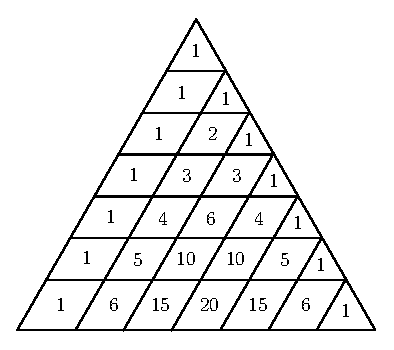
\includegraphics[scale=.7]{src/figures/m_151.eps}
\end{figure}
\centerline{\text{citarx $1$}}

pAsakxlana tirxBujavu
\begin{enumerate}
\item[{\rm 1)}] kaNaRgaLalilx aneVka riVtiya saMKAyx mAdari hoMdide.
\item[{\rm 2)}] sAvxBAvika saMKeyxgaLa motatx kaMDuhiDiyalu sahAyavAgide.
\item[{\rm 3)}] $(a+b)^n$ rUpada padagaLa visAtxra kaMDukoLaLxbahudu.
\item[{\rm 4)}] oMdu GaTaneya saMBavaniVyate kaMDuhiDiyabahudu.
\end{enumerate}

{\rm 1653} ralilx $(1+x)^n$ eMbudara vikeSxVpadalilx baruva saMKeyxgaLanunx kaMDuhiDiyuvu\-dakekx ``pAsakxlana tirxkoVna'' eMba saMKAyxpaTiTxyanunx vivarisidanu, I paTiTxyu hiMdeyeV ciVNAdalilx tiLiditutx. pAsakxlanigiMta hiMde yUroVpinalUlx aneVkaru idanunx parxsAtxpisidadxru. pAsakxlf idara viSayavAgi visheVSavAgi baredidadxriMda pAsakxlana tirxkoVna eMba samaMjasavalalxda hesaru niMtuhoVyitu.

pAsakxlf tirxBujavanunx ``laMbakoVna tirxBuja'' AkAradalilx matotxMdu riVtiyalilx bareyalu sAdhayx.
\begin{center}
\begin{tabular}{|>{$}c<{$}|>{$}c<{$}|>{$}c<{$}|>{$}c<{$}|>{$}c<{$}|>{$}c<{$}|>{$}c<{$}|>{$}c<{$}|}
\hline
1 & 1 & 1 & 1 & 1 & 1 & 1 & 1\\
\hline
1 & 2 & 3 & 4 & 5 & 6 & 7 & 8\\
\hline
1 & 3 & 6 & 10 & 15 & 21 & 28 & 36\\
\hline
1 & 4 & 10 & 20 & 35 & 56 & 84 & 120\\
\hline
1 & 5 & 15 & 35 & 70 & 126 & 210 & 330\\
\hline
1 & & & & & & &\\
\hline
\end{tabular} 
\end{center}
\begin{center}
citarx {\rm 2} 
\end{center}

\noindent
\textbf{pAsakxlana paTiTxyalilx aneVka visheVSa guNagaLive. citarx {\rm 2} raMte}
\begin{enumerate}
\item[{\rm 1)}] oMdaneya aDaDxsAlinalilx matutx oMdaneya kaMbasAlinalilx oMdu enunxvudu punarukitxyAgide.

\item[{\rm 2)}] eraDaneya kaMbasAlinalilx matutx eraDaneya aDaDxsAlinalilx karxmAgata saMKeyxgaLive.

\item[{\rm 3)}] mUraneya aDaDxsAlu matutx mUraneya kaMbasAlinalilx tirxBujAkAra saMKeyxgaLu EpaRTiTxve.

\item[{\rm 4)}]eraDaneV kaMbasAlina nAlakxneya aMkavu, nAlakxneya kaMbasAlina eraDaneya aMkavu, nAlukx Agide

\item[{\rm 5)}] eraDaneV aDaDxsAlina nAlakxneya aMkavu, nAlakxneya aDaDxsAlina eraDaneV aMkavu, nAlukx Agide.

\item[{\rm 6)}] mUraneya aDaDxsAlina, aidaneya aMkavu, aidaneya aDaDxsAlina mUraneya aMkavu, hadineYdu Agide.

\item[{\rm 7)}] eraDaneya aDaDxsAlina mUraneya aMkavu, mUraneya aDaDxsAlina eraDaneya aMkavu, mUru Agide.

\item[{\rm 8)}] eraDaneya aDaDxsAlina, nAlukx saMKeyxgaLa motatxvu, mUraneya aDaDxsAlina, nAlakxneya saMKeyxge sama.

$1, 2, 3, 4$ ra motatx {\rm 10}. idu mUraneya aDaDxsAlina saMKeyxyAgide.

\item[{\rm 9)}] nAlakxneya aDaDxsAlina aidu aMkagaLa motatx, aidaneya aDaDxsAlina aidaneya saMKeyxyAgide.

$1, 4, 10, 20, 35$ ra motatx {\rm 70}. idu aidaneV aDaDxsAlina aidaneV saMKeyxyAgide.

\item[{\rm 10)}]  vagARkAradalilxruva, nAlukx saMKeyxgaLanunx tegedukoMDare. 
$$
\begin{matrix}
6 && 10\\
& \rotatebox{45}{$\longleftrightarrow$} & \\
10 && 20
\end{matrix}
\qquad \text{mUle mUle {\rm 10} matutx {\rm 10} ra motatx {\rm 20} Agide.}
$$
\begin{center}
$\begin{matrix}
\text{ideV riVti} & 21 && 28\\
&& \rotatebox{45}{$\longleftrightarrow$} & \\
& 56 && 84
\end{matrix}$
\quad \text{mUle mUle {\rm 56} matutx {\rm 28} ra motatx {\rm 84}}\\[-0.55cm]
\text{~~ Agide.}
\end{center}

\item[{\rm 11)}] mUlemUlegaLalilxruva saMKeyxgaLanunx gamanisidAga divxpadoVkitxya visatxraNe\-yiMda saMKAyx sahaguNakagaLeMdu tiLidubarutatxde.
$$
\begin{matrix}
1\\
1 & 1\\
1 & 2 & 1\\
1 & 3 & 3 & 1\\
1 & 4 & 6 & 4 & 1 
\end{matrix}
\qquad \text{ivugaLelAlx saMKAyx guNAMkagaLu}
$$

\item[{\rm 12)}] idaralilx parxtiyoMdu saMKeyxyU, adara meVliruva saMKeyxge A (eraDaneya) saMKeyxya sAlinalilx adara eDakikxruva saMKeyxgaLanenxlAlx seVrisuvudariMda doreyutatxde.

udA: {\rm 4} neV sAlina  $10=6+3+1$ {\rm 5} neV sAlina  $35=20+10+4+1$

\item[{\rm 13)}] samabAhu tirxkoVnagaLAguvaMte kaNaRreVKegaLanenxLedare, A kaNaRreVKegaLa meVle baruva saMKeyxyu $(1+x)^n$ eMbudara vikeSxVpagaLanunx koDutatxve
\begin{flalign*}
\text{udA:} \quad (1+x)^4 &=1+4x+6x^2+4x^3+x^4 &\\
 (1+x)^5 &=1+5x+10x^2+10x^3+5x^4+x^5
\end{flalign*}

\item[{\rm 14)}] `PiboVnAkikx sherxVNi' ya saMKeyxgaLanunx kaMDukoLaLxlu sahAyavAgide.

\item[{\rm 15)}] vikalapxgaLa saMKeyxyanunx neVravAgi heVLabahudu.
\end{enumerate}


